% Ubah kalimat sesuai dengan judul dari bab ini
\chapter{PENGUJIAN DAN EVALUASI}

% Ubah konten-konten berikut sesuai dengan yang ingin diisi pada bab ini

\section{Skenario Pengujian}

Pengujian Siffars dilakukan dengan menggunakan PC yang memiliki spesifikasi GPU GTX1660 dan prosesor I7 lalu PC
tersebut diletakkan di sekretariat Departemen Teknik Komputer FTEIC-ITS. Selanjutnya beberapa tenaga kependidikan
Departemen Teknik Komputer FTEIC - ITS akan disimpan wajahnya dalam \texit{database} untuk digunakan dalam sistem deteksi Siffars.

\section{Evaluasi Pengujian}

Dari pengujian yang telah dibuat, didapatkan relevansi antara banyaknya data wajah tiap individu yang disimpan dalam database,
akurasi kemiripan tiap-tiap individu dan lama waktu yang dibutuhkan untuk dapat mendeteksi kemiripan tiap-tiap individu.

Semakin banyak wajah yang disimpan untuk tiap individu akan menghasilkan akurasi yang semakin tinggi untuk pendeteksian tingkat kemiripan,
namun juga akan membuat waktu pemrosesan untuk pendeteksian kemiripan wajah semakin lama. Begitupun sebaliknya,
semakin sedikit wajah yang disimpan untuk tiap individu akan menghasilkan akurasi yang semakin rendah untuk pendeteksian tingkat kemiripan,
namun juga akan membuat waktu pemrosesan untuk pendeteksian kemiripan wajah semakin cepat. Maka dari itu diperlukan
\texit{tunning} yang sesuai agar mendapatkan akurasi yang tinggi dan waktu pemrosesan yang cepat.

\begin{figure} [p] \centering
    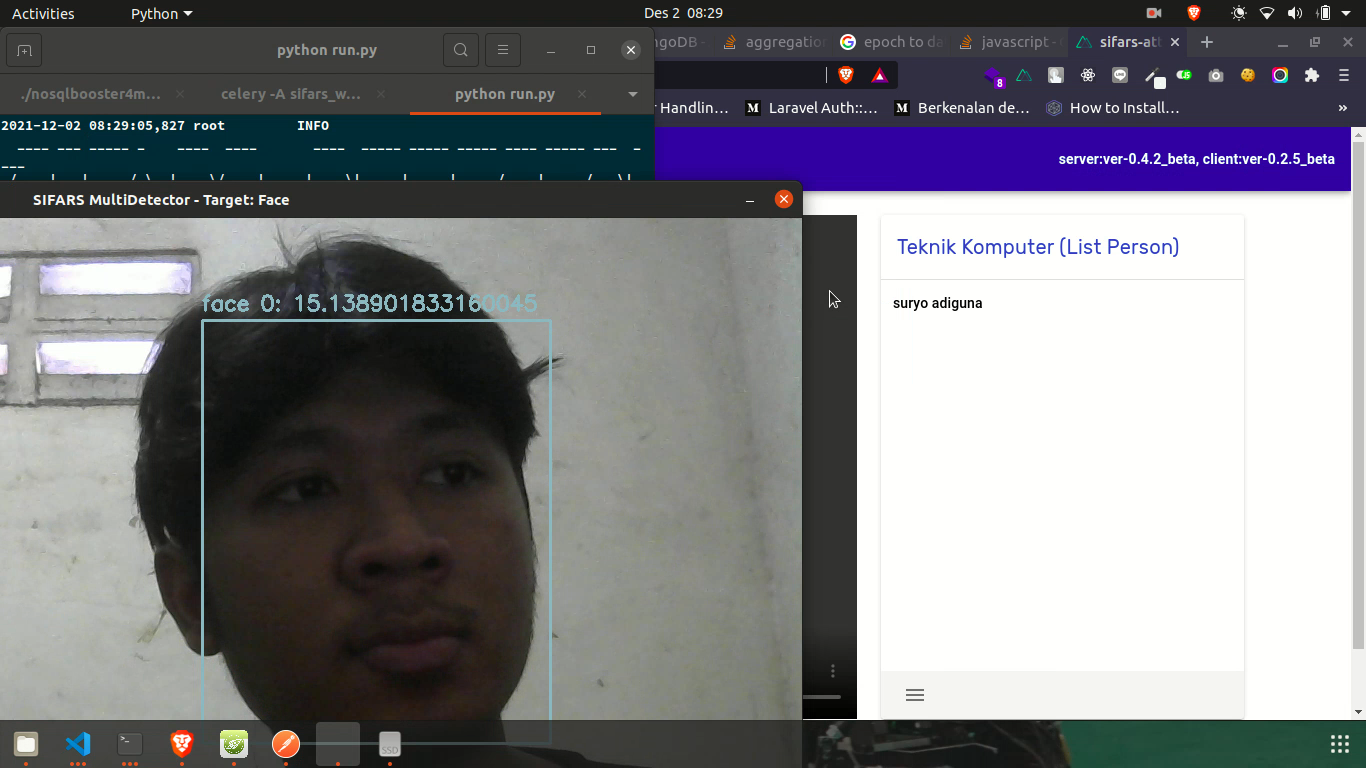
\includegraphics[scale=0.2]{gambar/demo1.png}
    \caption{Pengujian terhadap salah satu anggota kelompok (terdeteksi dan dikenali)}
    \label{fig:SfDemo1}
  
    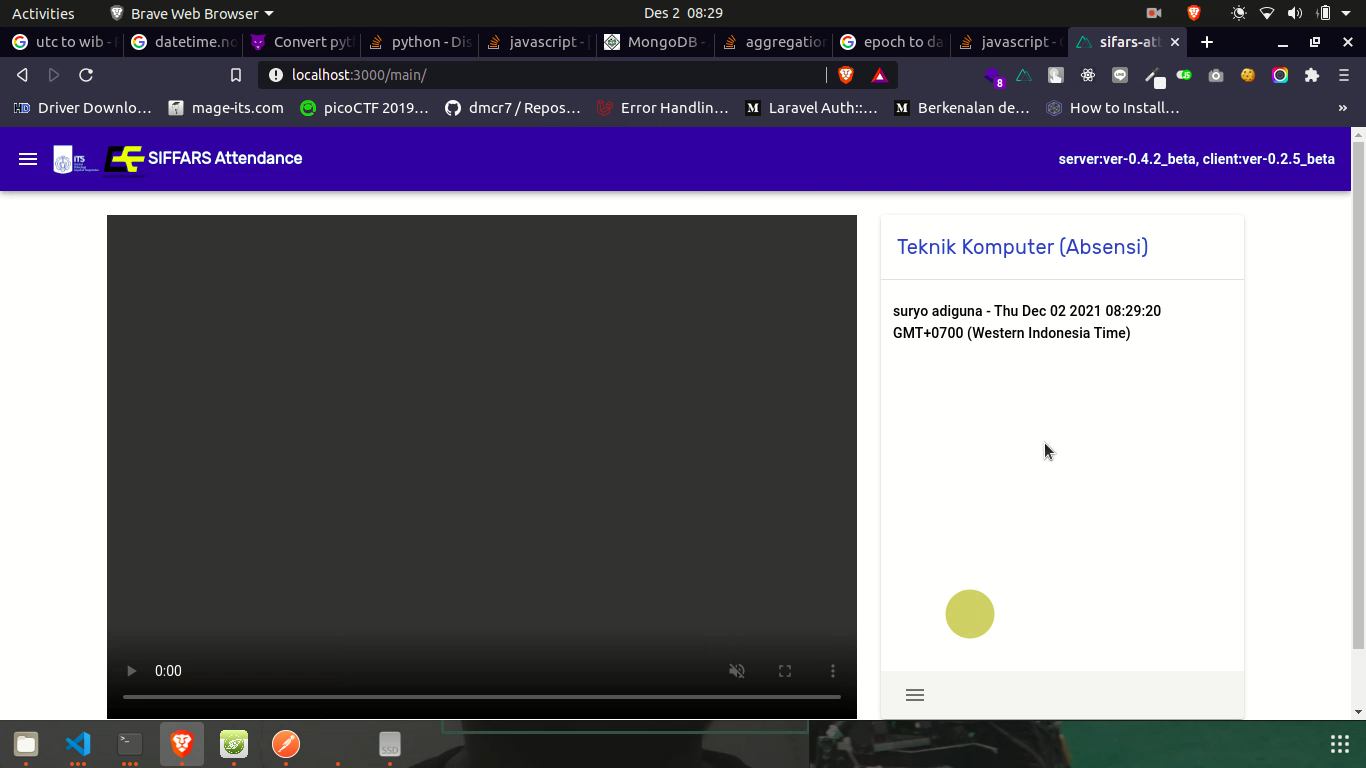
\includegraphics[scale=0.2]{gambar/demo2.png}
    \caption{Pengujian terhadap salah satu anggota kelompok (absensi tercatat)}
    \label{fig:SfDemo2}    
  \end{figure}

\begin{figure} [p] \centering
    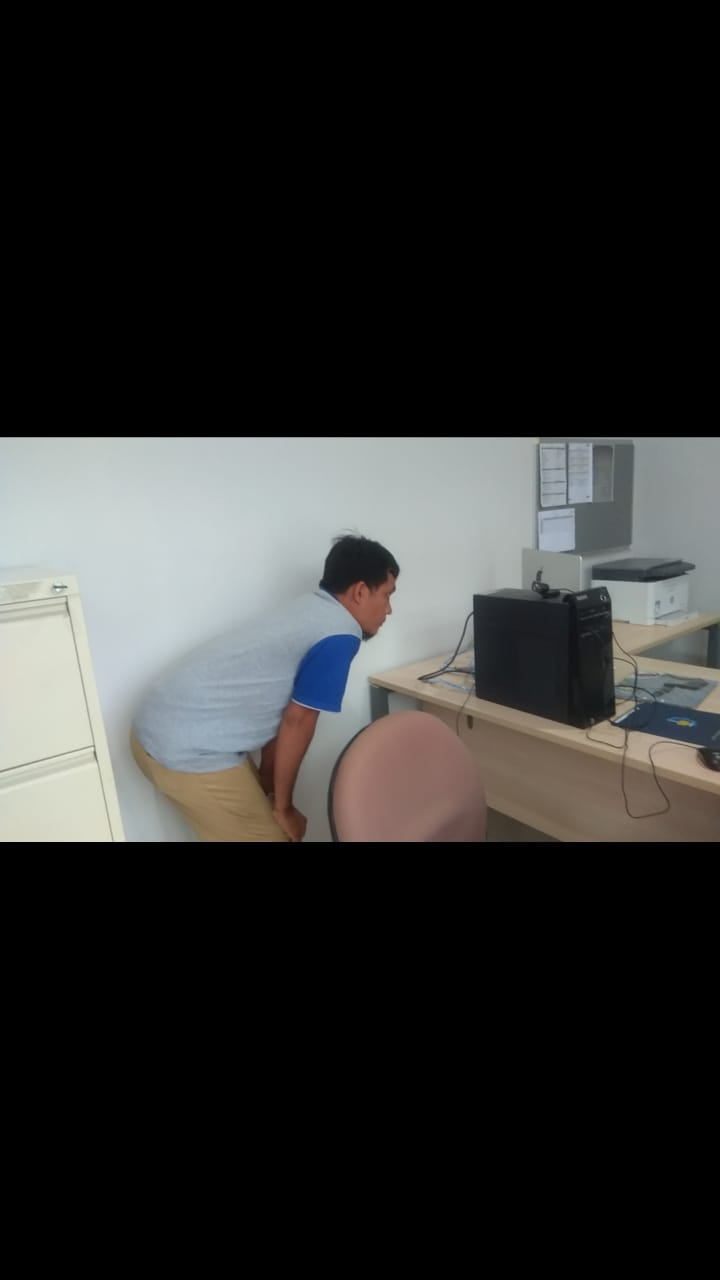
\includegraphics[scale=0.2]{gambar/masaris.jpeg}
    \caption{Pengujian terhadap salah satu tendik}
    \label{fig:SfMasaris}    
\end{figure}

\begin{figure} [p] \centering
    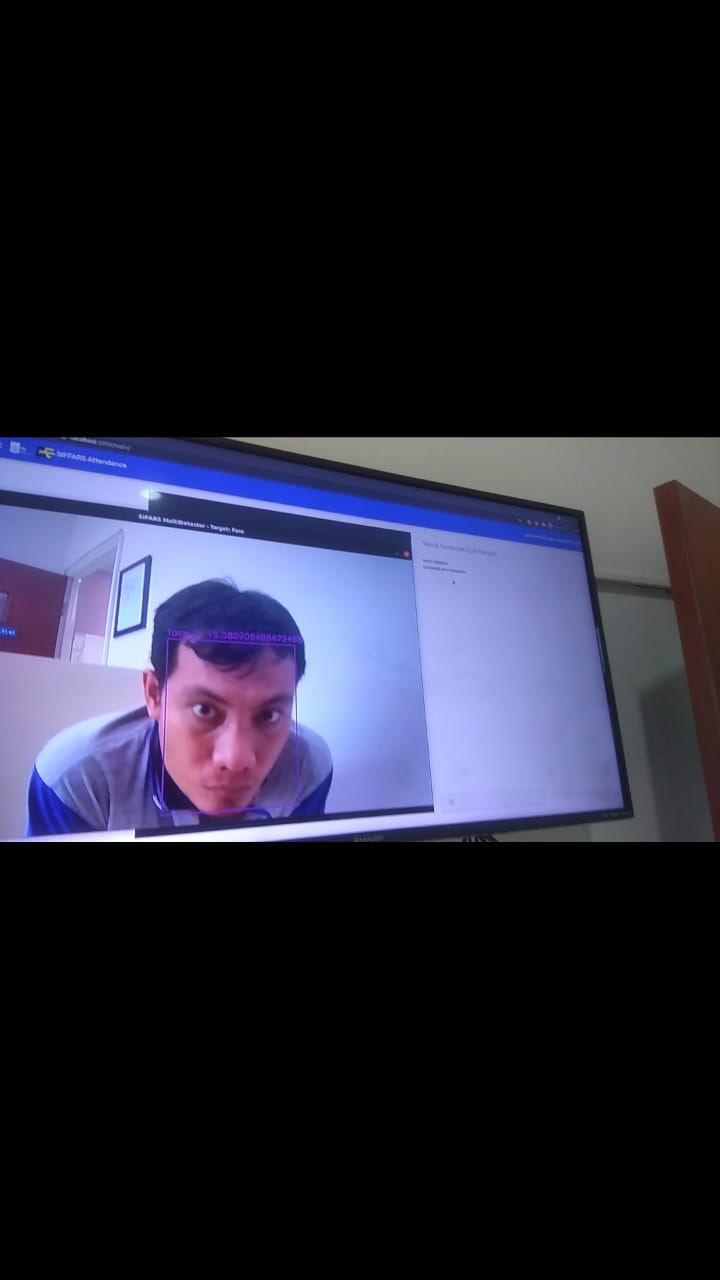
\includegraphics[scale=0.2]{gambar/masarisdetect0.jpeg}
    \caption{Pengujian terhadap salah satu tendik (terdeteksi dan dikenali)}
    \label{fig:SfMasarisdetect0}
\end{figure}

\begin{figure} [p] \centering
    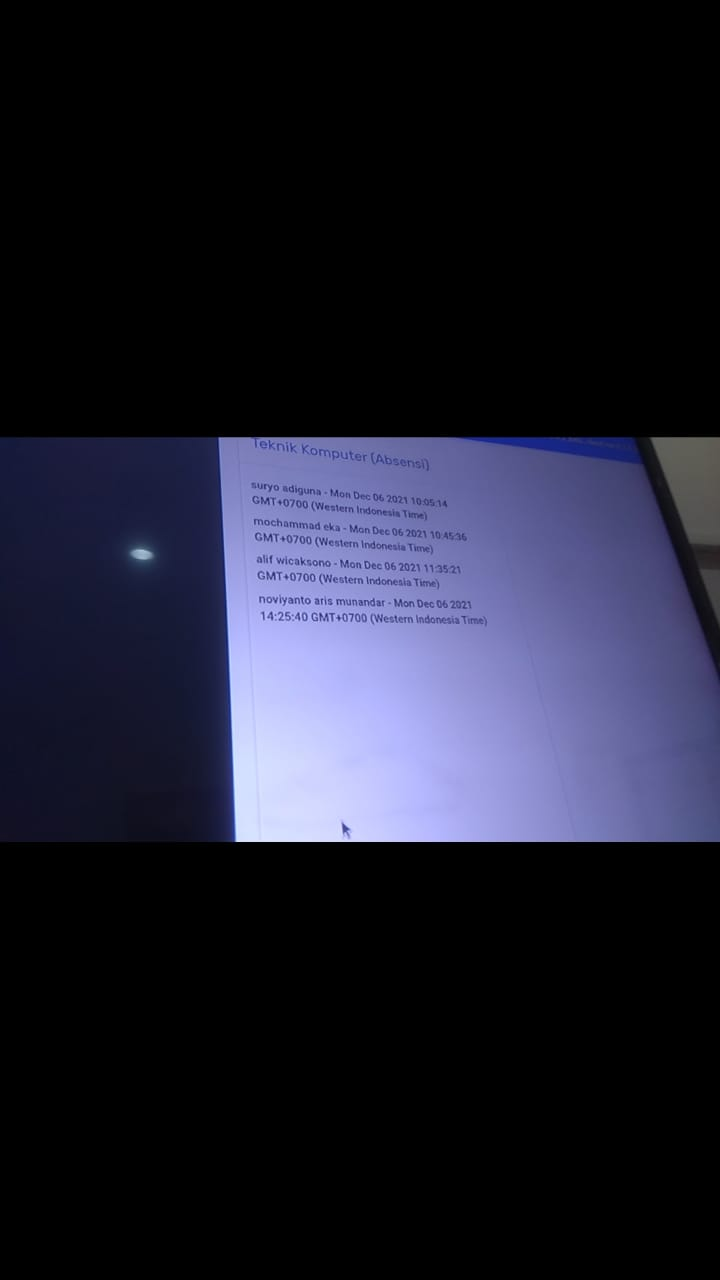
\includegraphics[scale=0.2]{gambar/masarisdetect.jpeg}
    \caption{Pengujian terhadap salah satu tendik (absensi tercatat)}
    \label{fig:SfMasarisdetect}
\end{figure}

\begin{figure} [p] \centering
    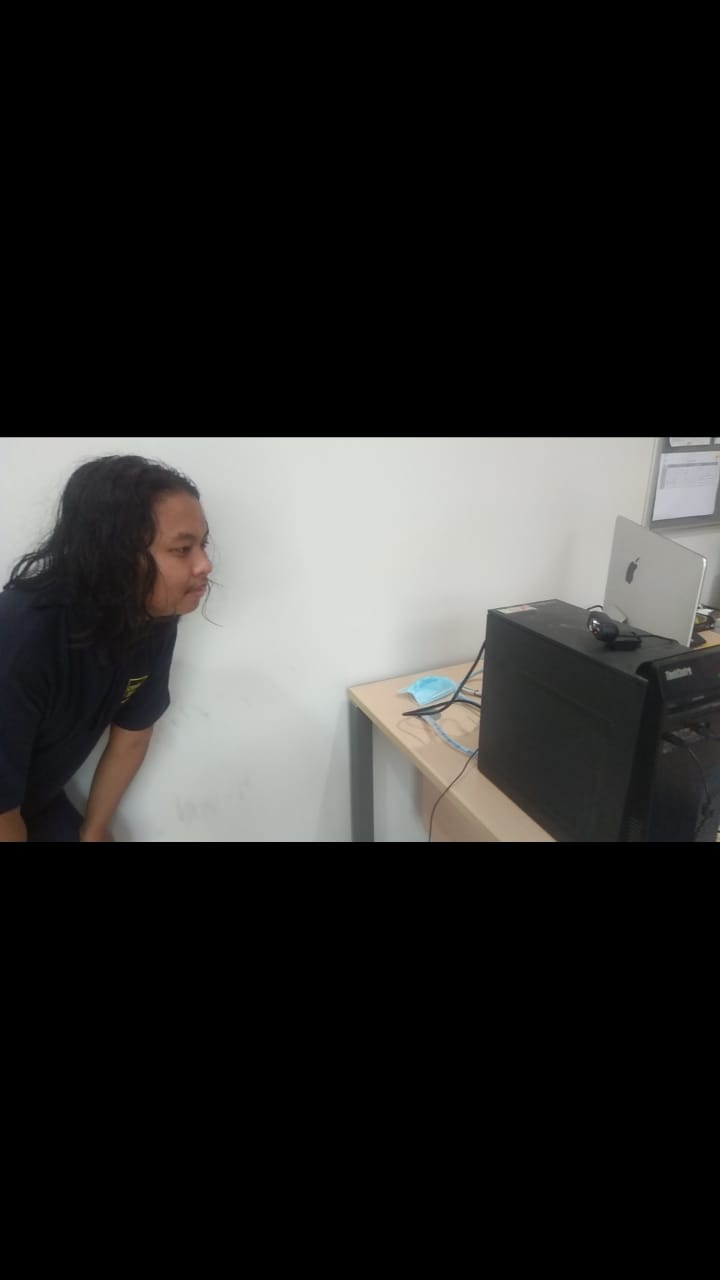
\includegraphics[scale=0.2]{gambar/ekadetect.jpeg}
    \caption{Pengujian terhadap salah satu mahasiswa}
    \label{fig:SfEka}
\end{figure}

\begin{figure} [p] \centering
    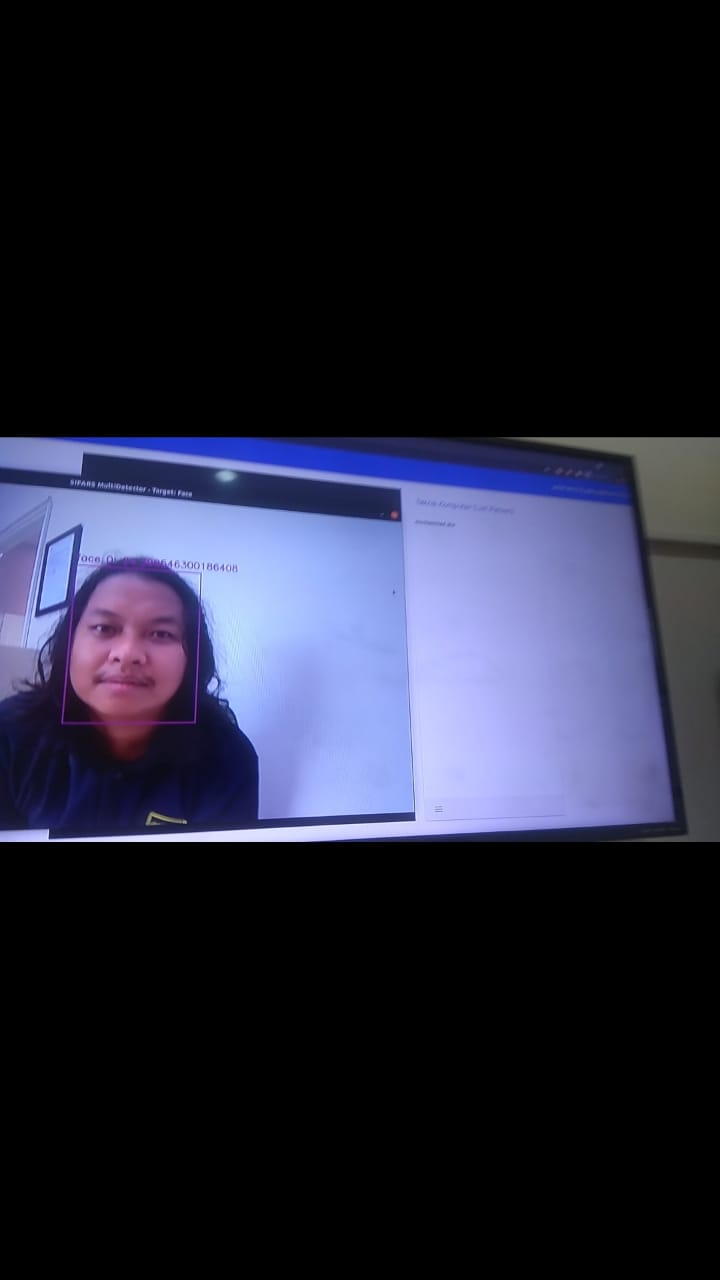
\includegraphics[scale=0.2]{gambar/ekadetect0.jpeg}
    \caption{Pengujian terhadap salah satu mahasiswa}
    \label{fig:SfEkadetect0}
\end{figure}

% % Contoh input konten dari file terpisah
% % Contoh pembuatan tabel
\begin{longtable}{|l|l|l|}
  % Keterangan dari tabel yang dibuat
  \caption{Hasil Pengukuran Energi dan Kecepatan}
  % Label referensi dari tabel yang dibuat
  \label{tb:EnergiKecepatan}\\
  % Isi dari tabel yang dibuat
  \hline
  \rowcolor[HTML]{C0C0C0}
  \textbf{Energi} & \textbf{Jarak Tempuh} & \textbf{Kecepatan} \\ \hline
  10 J & 1000 M & 200 M/s \\ \hline
  20 J & 2000 M & 400 M/s \\ \hline
  30 J & 4000 M & 800 M/s \\ \hline
  40 J & 8000 M & 1600 M/s \\ \hline
\end{longtable}


% % Contoh penggunaan referensi dari tabel yang dibuat
% Sesuai dengan hasil pada Tabel \ref{tb:EnergiKecepatan}, didapatkan bahwa energi yang \lipsum[26]
